\chapter{Evaluación y Resultados}

\par 
Luego de haber validado que el prototipo funcione correctamente se procede a iniciar con la etapa de evaluación del prototipo. Para validar si cumplimos con los estándares de la compañía SIGCSA se realizarán calibraciones a los siguientes dispositivos: 9 sensores o sondas del prototipo y 9 termómetros que actualmente utiliza la compañía para sus calibraciones en campo. Se utilizará el procedimiento operativo SIGCSA-PO-14 para la calibración para ello utilizaremos un termómetro patrón como referencia y la temperatura de nominal será indicada por un bloque de baño seco, para ambos equipos ver imagen 1.25.  Las temperaturas seleccionadas para las calibraciones serán: -10.00 C, 0.00 C, 10.00 C, 30.00 C y 50.00 C. En el Anexo 4 se pueden ver los detalles de las pruebas. En la próxima sección se indican los resultados de las pruebas realizadas.

\section{Resultados}

\par 
En esta sección se procederá a realizar un análisis de los resultados obtenidos de las calibraciones. Las calibraciones fueron ejecutadas por personal de la división de operaciones de SIGCSA. Los aspectos tomados en consideración para dichas calibraciones son las siguientes: Las calibraciones serán de un sensor de nuestro prototipo y un termómetro de campo de SIGCSA, ambos tomaran como referencia al termómetro patrón. Se realizarán 5 pruebas en distintas temperaturas y se tomarán 10 minutos para que la temperatura de todos los dispositivos se estabilicen y 10 minutos para la calibración, en esos 10 minutos se capturará el valor indicando por todos los dispositivos cada minuto. Una vez realizada las 5 pruebas se procede a utilizar un sensor de temperatura diferente para nuestro prototipo y un termómetro de campo diferente y nuevamente se realizan las mismas 5 pruebas con las mismas temperaturas. Se evaluarán 9 sensores, 5 pruebas cada uno, por lo que tenemos un total de 45 pruebas. A continuación se presentan dichos resultados: 

\subsection{Resultados obtenidos por el prototipo a -10.00 C}

\begin{figure}[H]
	\centering
	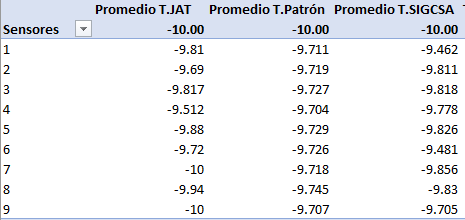
\includegraphics[width=0.5\linewidth]{resultados2.png}
	\caption{Tabla de Promedios de Temperaturas de prototipo y termómetros a -10.00 C}
\end{figure}

\par \noindent 
Los resultados de las pruebas son alentadores, en donde tomamos las 10 mediciones capturadas por el termómetro patrón, termómetro de campo de SIGCSA y nuestro prototipo, luego se procede a calcular sus respectivos promedios, ver figura 4.1. Con estos valores podemos realizar la siguiente gráfica:

\begin{figure}[H]
	\centering
	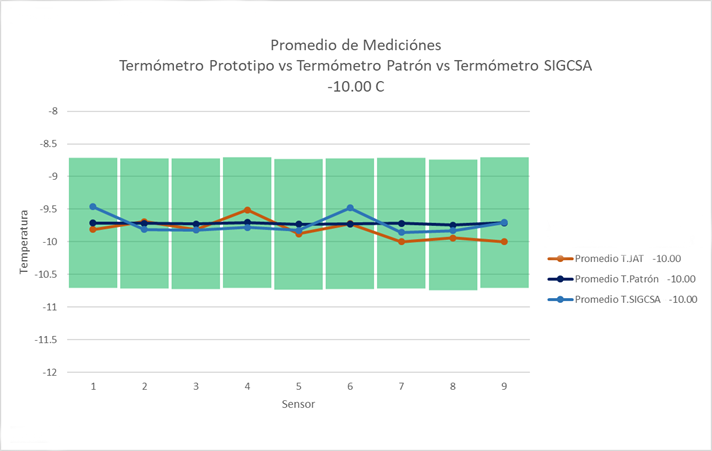
\includegraphics[width=0.6\linewidth]{resultados1.png}
	\caption{Gráfica de Promedios de Temperaturas de prototipo y termómetros a -10.00 C}
\end{figure}

\par \noindent
En la figura 4.2, podemos apreciar la línea del termómetro patrón con un color azul oscuro. Los termómetros de campo de SIGCSA con una línea azul claro y los sensores de nuestro prototipo en naranja oscuro. Como hemos utilizado el mismo termómetro patrón se pude notar que su línea es más uniforme. Las barras verdes representan el área en donde el termómetro de campo de SIGCSA y nuestro el sensor del prototipo se debe encontrar para cumplir con los estándares de la compañía. Tanto nuestro prototipo como el termómetro de campo cumplen. Se realizó el mismo procedimiento pero esta vez la temperatura a 0.00 C



\subsection{Resultados obtenidos por el prototipo a -10.00 C}

\begin{figure}[H]
	\centering
	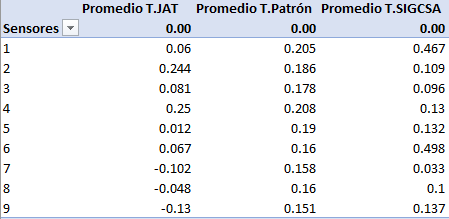
\includegraphics[width=0.5\linewidth]{resultados3.png}
	\caption{Tabla de Promedios de Temperaturas de prototipo y termómetros a 0.00 C}
\end{figure}

\par \noindent 
Los resultados obtenidos por las calibraciones, ver Anexo 4 , son utilizados para calcular la temperatura promedio del termómetro patrón, los nueve termómetros de campo de SIGCSA y los sensores de temperatura del prototipo, ver figura 4.3 y con estos valores podemos realizar la siguiente gráfica:

\begin{figure}[H]
	\centering
	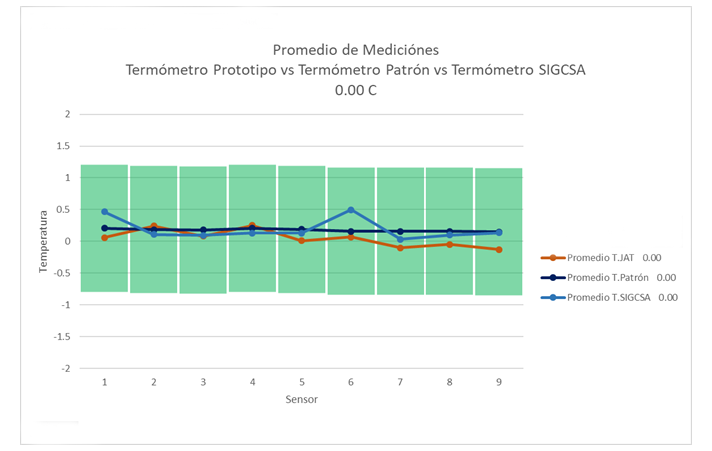
\includegraphics[width=0.8\linewidth]{resultados4.png}
	\caption{Grafica de Promedios de Temperaturas de prototipo y termómetros a 0.00 C}
\end{figure}

\par \noindent
Como podemos ver nuevamente los sensores del prototipo y los termómetros de campo de SIGCSA se encuentran en el rango aceptable para la compañía. Pero si comparamos la figura 4.4 y 4.2 podemos observar que ciertos sensores del prototipo y termómetros de campo, el error de ellos se empieza a ampliar con respecto al termómetro patrón. A continuación los resultados a 10.00 grados Celsius.


\subsection{Resultados obtenidos por el prototipo a 10.00 C}

\begin{figure}[H]
	\centering
	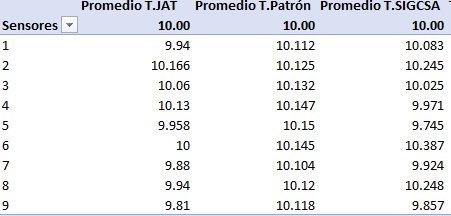
\includegraphics[width=0.5\linewidth]{resultados5.png}
	\caption{Tabla de Promedios de Temperaturas de prototipo y termómetros a 10.00 C}
\end{figure}

\par \noindent 
Los resultados obtenidos por las calibraciones, ver Anexo 4 , son utilizados para calcular la temperatura promedio del termómetro patrón, los nueve termómetros de campo de SIGCSA y los sensores de temperatura del prototipo, ver figura 4.5 y con estos valores podemos realizar la siguiente gráfica:

\begin{figure}[H]
	\centering
	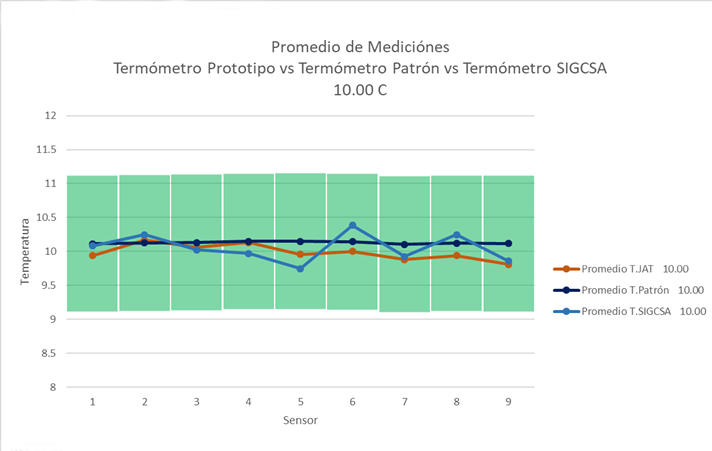
\includegraphics[width=0.8\linewidth]{resultados6.png}
	\caption{Grafico de Promedios de Temperaturas de prototipo y termómetros a 10.00 C}
\end{figure}

\par \noindent
Nuevamente tanto el prototipo como los termómetros de campo de SIGCSA se encuentran en el rango de aceptación de la compañía. Sin embargo si comparamos la figura 4.2 y la 4.6 podemos observar que a medida que la temperatura va subiendo los termómetros de campo de SIGCSA comienzan a perder exactitud con respecto al termómetro patrón. El más pronunciado de todos es el termómetro de campo #5, el cual se encontraba muy cerca del termómetro patrón en -10.00 grados Celsius pero ahora se alejado considerablemente de la medición del termómetro patrón. Ahora seguimos con los resultados obtenidos a 30.00 grados Celsius.


\subsection{Resultados obtenidos por el prototipo a 30.00 C}

\begin{figure}[H]
	\centering
	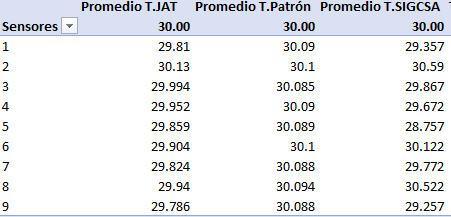
\includegraphics[width=0.5\linewidth]{resultados7.png}
	\caption{Tabla de Promedios de Temperaturas de prototipo y termómetros a 30.00 C}
\end{figure}

\par \noindent 
Los resultados obtenidos por las calibraciones, ver Anexo 4 , son utilizados para calcular la temperatura promedio del termómetro patrón, los nueve termómetros de campo de SIGCSA y los sensores de temperatura del prototipo, ver figura 4.7 y con estos valores podemos realizar la siguiente gráfica:

\begin{figure}[H]
	\centering
	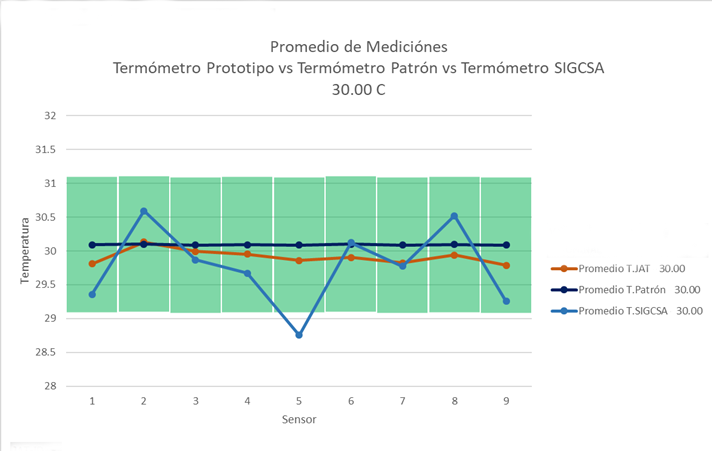
\includegraphics[width=0.6\linewidth]{resultados8.png}
	\caption{Grafica de Promedios de Temperaturas de prototipo y termómetros a 30.00 C}
\end{figure}

\par \noindent
La figura 4.8 en la gráfica el termómetro de campo de SIGCSA, el numero 5 a salido del error permitido con respecto al patrón. Adicional los termómetros 1, 2, 8 y 9 también se encuentran con un error mayor de 0.5 grados con respecto al  patrón. Esto indica que los termómetros de campo comenzarán a indicar valores de temperatura inexactos a medida que sube la temperatura del medio isotermo a calibrar. Sin embargo los sensores del prototipo aún mantienen las mismas lecturas con respecto al patrón. A continuación son los resultados a una temperatura de 50.00 grados Celsius.


\subsection{Resultados obtenidos por el prototipo a 50.00 C}

\begin{figure}[H]
	\centering
	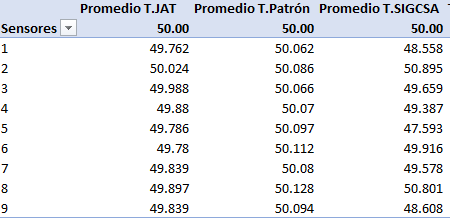
\includegraphics[width=0.5\linewidth]{resultados9.png}
	\caption{Tabla de Promedios de Temperaturas de prototipo y termómetros a 30.00 C}
\end{figure}

\par \noindent 
Los resultados obtenidos por las calibraciones, ver Anexo 4 , son utilizados para calcular la temperatura promedio del termómetro patrón, los nueve termómetros de campo de SIGCSA y los sensores de temperatura del prototipo, ver figura 4.9 y con estos valores podemos realizar la siguiente gráfica:

\begin{figure}[H]
	\centering
	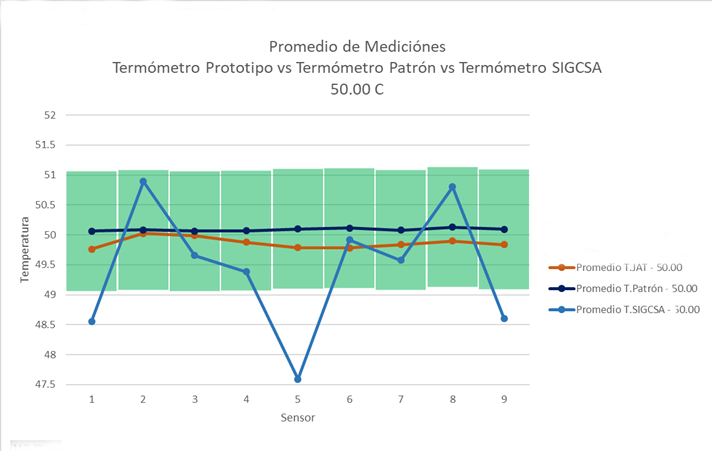
\includegraphics[width=0.6\linewidth]{resultados10.png}
	\caption{Grafica de Promedios de Temperaturas de prototipo y termómetros a 30.00 C}
\end{figure}

\par \noindent
En la última gráfica, figura 4.10. Dos de los termómetros de campo previamente mencionados salen del error máximo permitido (#1 y #9) y el termómetro de campo #6 se aleja cada vez más del patrón. Los termómetros de campo #2 y #8 se encuentran muy cercanos del error máximo. Los sensores de temperatura del prototipo aún siguen manteniendo un margen de error aceptable; sin embargo, ya a esta temperatura podemos encontrar un aumento del error de medición con respecto al patrón específicamente en el sensor 1 y 5.


\clearpage


\section{Conclusiones}

\par \noindent
Con la desarollo de nuestro prototipo y las pruebas realizadas se ha llegado a las siguientes conclusiones:

\begin{itemize}
	\item Nuestro prototipo cumple con los estándares de la compañía SIGCSA. 
	
	\item Los sensores de temperatura utilizados en el prototipo fueron comparados con termómetros de campo de SIGCSA, los cuales ya tienen un año de uso. Por lo que es necesario nuevamente pruebas de los sensores del prototipo en un plazo de un año.
	
	\item La aplicación se conecta por bluetooth al prototipo más hace falta mejorar la comunicación de radiofrecuencia para una comunicación entre 2 o más prototipos de manera confiables.
	
	\item El prototipo puede operar de manera continua con una alimentación a través de USB y por 3 horas utilizando la batería interna.
\end{itemize}

\clearpage

\mbox{}
\clearpage


\section{Recomendaciones}

\begin{itemize}
	\item Mejorar el sistema de comunicación de radiofrecuencia; considerar utilizar otros módulos de radiofrecuencia.
		
	\item Mejorar la eficiencia de la batería o considerar utilizar una batería más grande para obtener por lo menos 8 horas de operación del prototipo. 
	
	\item Por recomendación del personal sería bueno que la base de datos de la aplicación se pueda sincronizar con la base de datos MYSQL de la compañía. 
\end{itemize}

\clearpage

\mbox{}
\clearpage

